\documentclass[12pt,a4paper]{article}
\usepackage[utf8]{inputenc}
\usepackage[OT1]{fontenc}
\usepackage{amsmath}
\usepackage{amsfonts}
\usepackage{amssymb}
\usepackage{graphicx}
\usepackage{tikz}
\usepackage{pgfplotstable}
\usepackage{mathtext}

\usepackage[T1]{fontenc}
\usepackage[utf8]{inputenc}
\usepackage[english, bulgarian, russian]{babel}

\usepackage{tikz}
\usepackage{pgfplots}
\usepackage{indentfirst}
\usepackage[export]{adjustbox}
\usepackage{multirow}
\usepackage{geometry} \geometry{verbose,a4paper,tmargin=2cm,bmargin=2cm,lmargin=1.5cm,rmargin=1.5cm}

\graphicspath{{Images/}}
\usepackage[left=2cm,right=2cm,top=2cm,bottom=2cm]{geometry}
\usepackage{wrapfig}
\usepackage{setspace}
\usepackage{indentfirst}
\usepackage{subfigure}


\begin{document}

\begin{titlepage}
  \begin{center}
    \huge
    Московский Физико-технический Институт
    
    (Национальный исследовательский университет)
    \vspace{0.5cm}

   
    \vspace{0.25cm}
 
    \vfill
 
    \vfill

    \textsc{\bf{Отчет о выполнении работы 3.4.2}}\\[3mm]
    
    {\LARGE Закон Кюри-Вейсса}
  \bigskip
    \vfill
    
\end{center}
\vfill
\begin{flushright}

    Выполнили студентки 2 курса
    
    ФБМФ, группа Б06-103

    Попеску Полина
    
    
    Фитэль Алёна

\end{flushright}
\bigskip


\vfill

\begin{center}
  Долгопрудный, 2022 г.
\end{center}
\end{titlepage}


\section{Историческая справка}

Ферромагнетики обладают свойством намагничиваться даже в слабых магнитных полях. Впервые количественную теорию ферромагнетизма разработал французский физик Вейсс в 1907 году. В настоящей работе для изучения температурной зависимости магнитной восприимчивости ферромагнетика выше точки Кюри (то есть в парамагнитной области) используется закон Кюри-Вейса (который назван так по аналогии с законом Кюри для парамагнетиков).

Закон выражается следующей математической формулой:

 \begin{equation}\label{QW}
 \chi ={\frac  {C}{T-\Theta_p}} \sim \frac{1}{T - \Theta_p}, 
 \end{equation}
 
где $ \chi  $ — магнитная восприимчивость, $ С $ — постоянная Кюри, зависящая от вещества, $ T $ — абсолютная температура в кельвинах, $ \Theta_p  $ — парамагнитная температура Кюри, К.

\section{Теоретическое введение}

При повышении температуры $ Т $ возрастает дезориентирующее действие теплового движения частиц, и магнитная восприимчивость парамагнетиков
убывает, в простейшем случае (в постоянном магнитном
поле) - пo закону Кюри.

\begin{wrapfigure}{l}{0.3\linewidth} 
	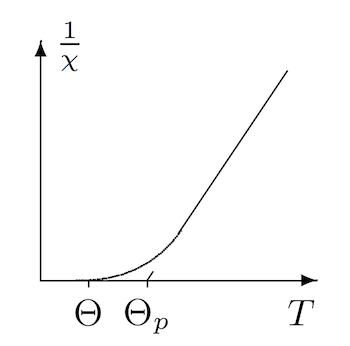
\includegraphics{342teorgraph.png}
	\caption{Теоретический график зависимости обратной магнитной восприимчивости от температуры}
\end{wrapfigure}

При $ Т \to 0 $ тепловое движение всё меньше препятствует магнитным моментам атомов ориентироваться в одном направлении при сколь
угодно слабом внешнем поле. В ферромагнетиках (под влиянием обменных сил) это происходит при понижении температуры не до абсолютного
нуля, а до температуры Кюри $ \Theta $, в котором добавка к температуре $ \Theta_p $ --- некая температура, называемая парамагнитной точкой Кюри. Она близка к $ \Theta $, но немного больше ее (см. рис.1). Оказывается, что у ферромагнетиков закон Кюри должен быть заменён законом Кюри-Вейсcа \eqref{QW}. Эта формула хорошо описывает поведение ферромагнитных  веществ после их перехода в парамагнитную фазу при заметном удалении температуры от 0 , но недостаточно точна при $ Т \approx \Theta$.

В нашей работе изучается температурная зависимость $ \chi(Т) $ гадолиния
при температурах выше точки Кюри. Выбор материала определяется
тем, что его точка Кюри лежит в интервале комнатных температур.

\section{Экспериментальная установка} 
\begin{figure}[h!]
	\centering
	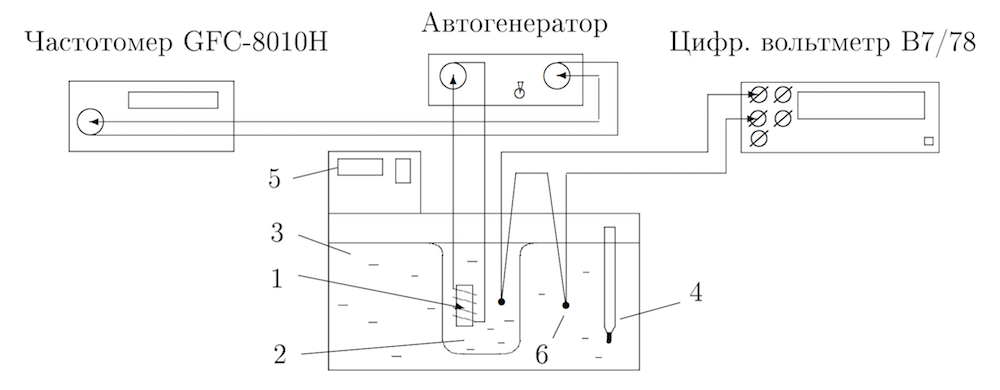
\includegraphics[width=\linewidth]{ust.png}
	\caption{Схема эксперементальной установки}
	\label{ust}
\end{figure}

Схема установки для проверки закона Кюри-Вейсса показана на рис. 2. Исследуемый ферромагнитный образец (гадолиний) расположен внутри пустотелой катушки самоиндукции, которая служит индуктивностью колебательного контура, входящего в состав $ LС $-автогенератора. 

Гадолиний является хорошим проводником электрического тока, а рабочая
частота генератора достаточно велика (50 кГц), поэтому для уменьшения
вихревых токов образец из готовлен из мелких кусочков размером 0,5 мм.
Катушка 1 с образцом помещена в стеклянный сосуд 2, залитый трансформаторным маслом. Масло предохраняет образец от окисления и способствует ухудшению электрического контакта между отдельными частичками образца. Кроме того, оно улучшает тепловой контакт между образцом и термостатируемой (рабочей) жидкостью 3 в термостате. Ртутный термометр 4 используется для приближенной оценки температуры.
При изменении температуры меняется магнитная восприимчивость образца
$ \chi $, а следовательно, самоиндукция катушки и период колебаний $ \tau $ автогенератора. Для измерения периода используется частотомер.

Закон Кюри- Вейсса справедлив, если выполнено соотношение

\begin{equation}\label{}
\dfrac{1}{\chi} \sim T - \Theta_p \sim \dfrac{1}{\tau^2 - \tau^2_0}
\end{equation}
где $ \tau_0 $ --- период колебаний без образца. 

Для нагрева используется термостат. Температура исследуемого образца всегда несколько отличается от температуры дистиллированной воды в сосуде. После того как вода достигла заданной температуры, идёт медленный процесс выравнивания температур образца и воды. Разность их температур контролируется с помощью медноконстантановой термопары 6 и цифрового вольтметра. Один из спаев термопары находится в тепловом контакте с образцом , а другой погружён в воду. Концы термопары подключены к цифровому вольтметру. Рекомендуется измерять период колебаний автогенератора в тот момент, когда указанная
разность температур становится $  \leq 0,5 \; ^\circ С $. Чувствительность термопары $ k= 24 $ град/мВ.

\section{Ход работы}

{\bf LC-контур: }$\tau_0 = 8.252 $ \si{\micro \second}


Так как нам нужно, чтобы разница была не более половины градуса, то мы вычисляем максимальное напряжение, при котором допустимо измерение:

\begin{equation}\label{}
U_m = \dfrac{T_d}{k} = \dfrac{0,5}{24} \approx 0,021 \un{мВ} 
\end{equation}

Теперь снимем показания вольтметра и частометра при температуре термостата равной 14 $ ^\circ C $, и проведем такой опыт при 14 разных температурах, повышая после каждого измерения температуру термостата на два градуса. При этом температуру образца будем считать по следующей формуле:

\begin{equation}\label{}
T_o = T_в + \varDelta Uk
\end{equation}


\begin{table}[h!]
\centering
\begin{tabular}{|c|c|c|c|c|c|}
\hline
\textbf{T, K} & \textbf{$\tau$, us} & \textbf{$\triangle$U, mV} & \textbf{$\sigma_{\tau}$} & \textbf{$T_{\text{обр}}$} & \textbf{$\sigma_{T_{\text{обр}}}$} \\ \hline
289           & 9,900              & -0,006                    & 0,050                    & 288,86                    & 0,1                                \\ \hline
291           & 9,800              & -0,027                    & 0,100                    & 290,35                    & 0,1                                \\ \hline
293           & 9,440              & -0,016                    & 0,010                    & 292,62                    & 0,1                                \\ \hline
295           & 9,060              & -0,019                    & 0,010                    & 294,54                    & 0,1                                \\ \hline
297           & 8,750              & -0,019                    & 0,005                    & 296,54                    & 0,1                                \\ \hline
299           & 8,610              & -0,015                    & 0,005                    & 298,64                    & 0,1                                \\ \hline
301           & 8,536              & -0,018                    & 0,002                    & 300,57                    & 0,1                                \\ \hline
303           & 8,488              & -0,019                    & 0,002                    & 302,54                    & 0,1                                \\ \hline
305           & 8,454              & -0,019                    & 0,002                    & 304,54                    & 0,1                                \\ \hline
307           & 8,429              & -0,018                    & 0,002                    & 306,57                    & 0,1                                \\ \hline
309           & 8,411              & -0,019                    & 0,001                    & 308,54                    & 0,1                                \\ \hline
311           & 8,396              & -0,019                    & 0,001                    & 310,54                    & 0,1                                \\ \hline
313           & 8,384              & -0,018                    & 0,001                    & 312,57                    & 0,1                                \\ \hline
\end{tabular}
\caption{Результаты измерений}
\end{table}

Посчитаем погрешности: 

$$
\sigma_{T_o} = \sqrt{\sigma_{T_в}^2 + \sigma_{dUk}^2}
$$
\begin{equation}\label{}
\sigma_{\tau^2 - \tau_0^2} = \dfrac{d(\tau^2 - \tau_0^2)}{d\tau}\sigma_\tau = 2\tau\sigma_\tau
\end{equation}
\begin{equation}\label{}
\sigma_{\frac{1}{\tau^2 - \tau_0^2}} = \dfrac{d\s{\dfrac{1}{\tau^2 - \tau_0^2}}}{d\tau}\sigma_\tau = \dfrac{2\tau}{{(\tau^2 - \tau_0^2)^2}}\sigma_\tau
\end{equation}

Построим графики зависимости величин $ \tau^2 - \tau_0^2 $ и $ \dfrac{1}{\tau^2 - \tau_0^2} $ от температуры образца.
\par

\vspace{1mm}
\begin{figure}[h!]
	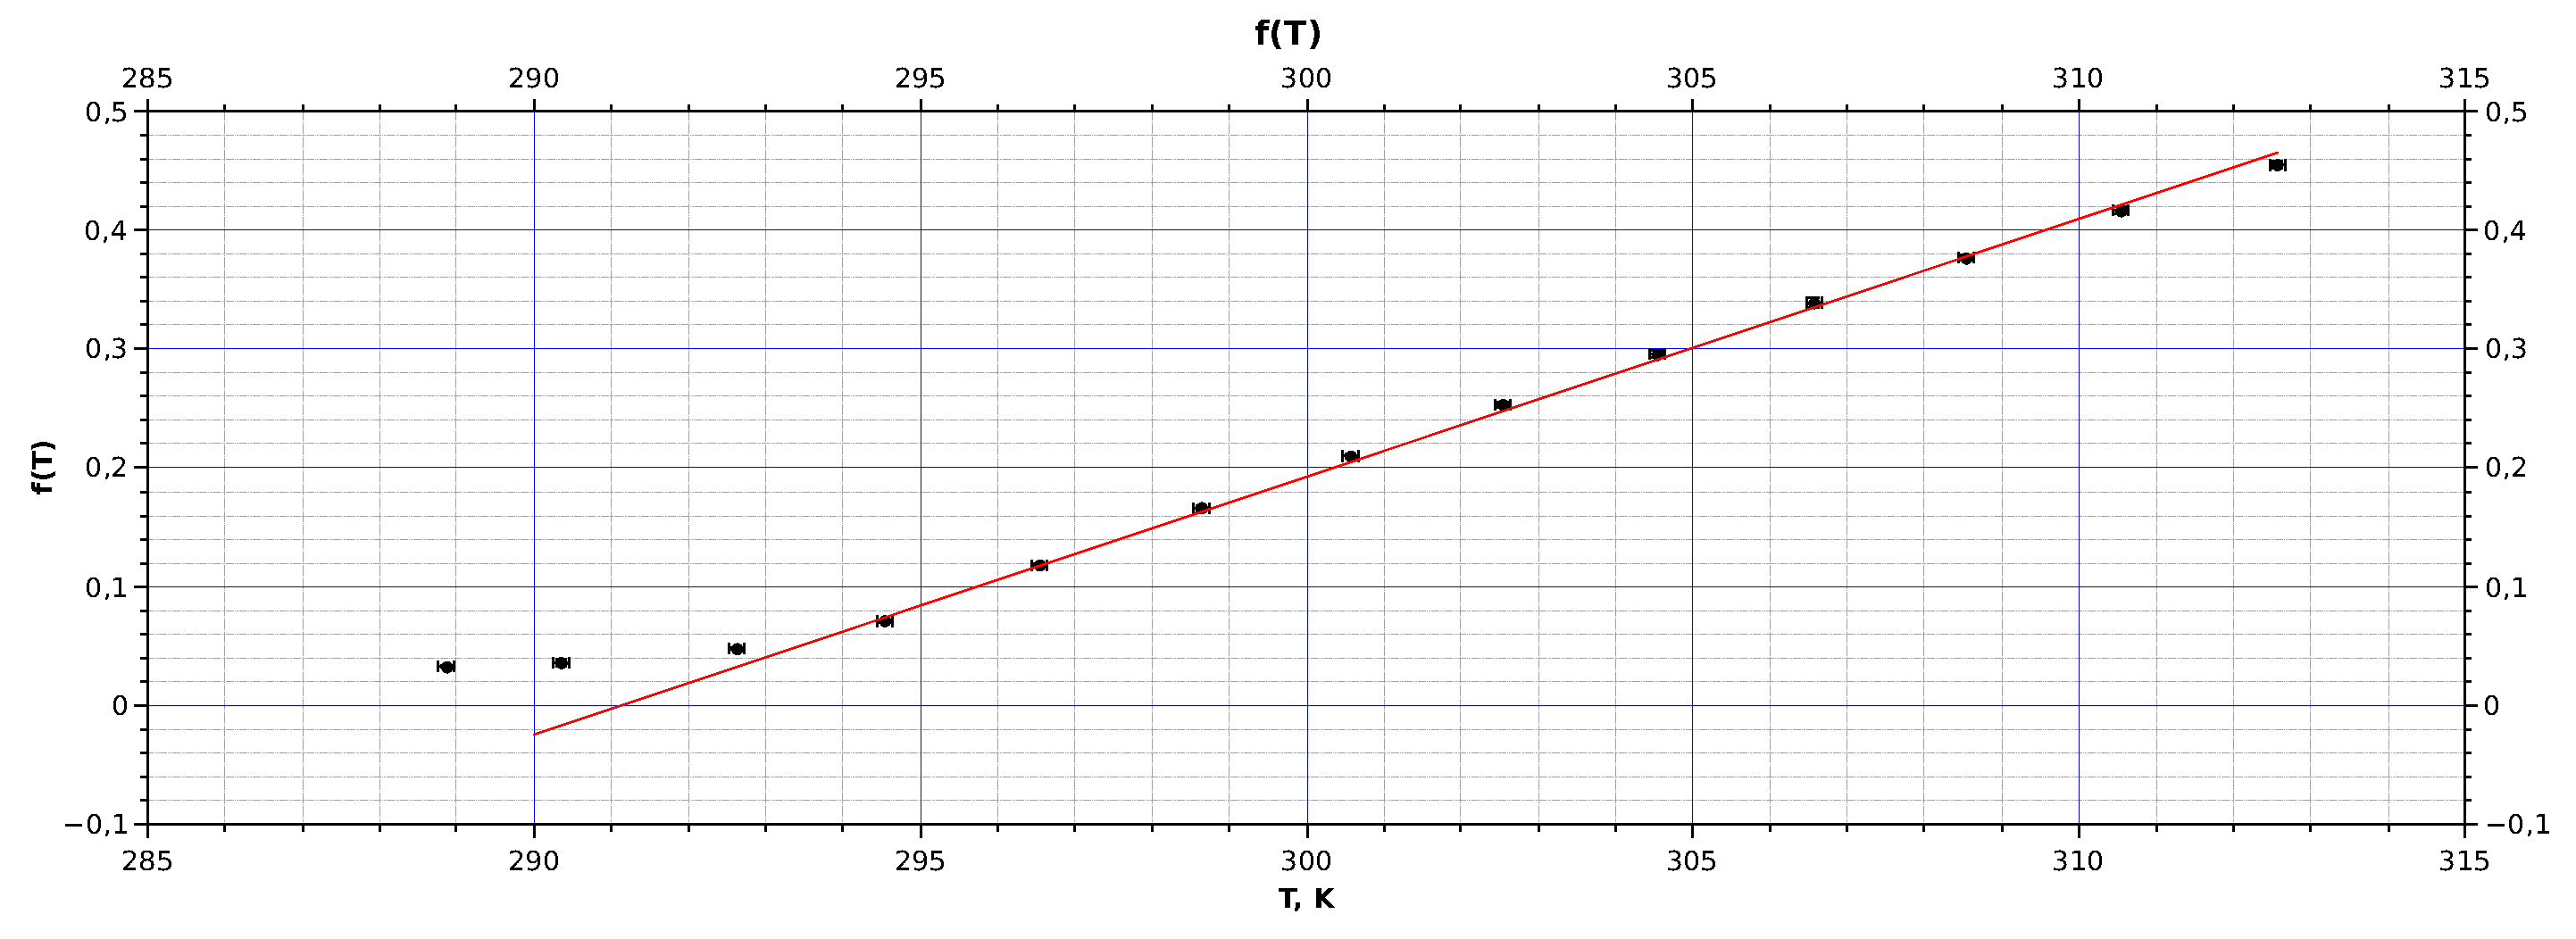
\includegraphics[scale=0.37]{Graph3.pdf}
	\caption{Зависимость $ \dfrac{1}{ \tau^2 - \tau_0^2} $ от температуры образца}
\end{figure}


Экстраполируя график к оси абсцисс мы полчили значение температуры точки Кюри равной $\Theta_K = (290,3 \pm 2,6) K \; (\varepsilon = 0,9 \%)$. Табличное значение -- $ \Theta = 293 К $.


\section{Вывод}

Исследуя гадолиний с помощью термостата, частотометра и вольтметра мы определили темперературу точки Кюри для гадолиния:

\begin{center}
	{\fbox{ $ \Theta_p = (290,3 \pm 2,6) K \; (\varepsilon = 0,9 \%)$}} \\
\end{center} 

С учетом погрешности погрешности посчитанное значение совпадает с табличным (293К).


\end{document}